26. $\cfrac{(x^2-4)(y-x+1)}{x-2}=0=0\Leftrightarrow\cfrac{(x-2)(x+2)(y-x+1)}{x-2}=0\Leftrightarrow
\begin{cases}\left[\begin{array}{l}x=-2,\\ y=x-1.\end{array}
ight.\\ x
eq2\end{cases}$
$$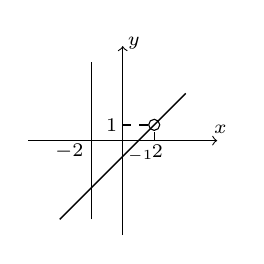
\begin{tikzpicture}[scale=0.2]
\tikzset {line01/.style={line width =0.5pt}}
\tikzset{line02/.style={line width =1pt}}
\tikzset{line03/.style={dashed,line width =0.5pt}}
%\filldraw [black] (0,0) circle (1pt);
\draw [->] (-6,0) -- (6,0);
\draw [->] (0,-6) -- (0,6);
\draw[line01] (-2,-5) -- (-2,5);
\draw[line01] (-4,-5) -- (4,3);
\draw (6.2,0.7) node {\scriptsize $x$};
\draw (-3.4,-0.7) node {\scriptsize $-2$};
\draw (2.2,-0.7) node {\scriptsize $2$};
\draw (-0.7,1) node {\scriptsize $1$};
\draw (1.1,-1) node {\tiny $-1$};
\draw[line03] (2,0) -- (2,1);
\draw[line03] (0,1) -- (2,1);
\draw (0.7,6.2) node {\scriptsize $y$};
\draw (2,1) circle (10pt);
\end{tikzpicture}$$
